% !TEX TS-program = pdflatexmk
% !BIB TS-program = bibtex

\documentclass[12pt, a4paper, twoside]{book}
\usepackage{import}
\subimport{../}{preamble}
\ExecuteBibliographyOptions{articletitle=false}
\standalonetrue
\onehalfspacing
\begin{document}

\begin{singlespace}
\chapter{Understanding and Applying Single Tip Plasmonics}
\end{singlespace}

%\AddToShipoutPictureBG*{ \AtPageUpperLeft{ \put(0,-240)
%{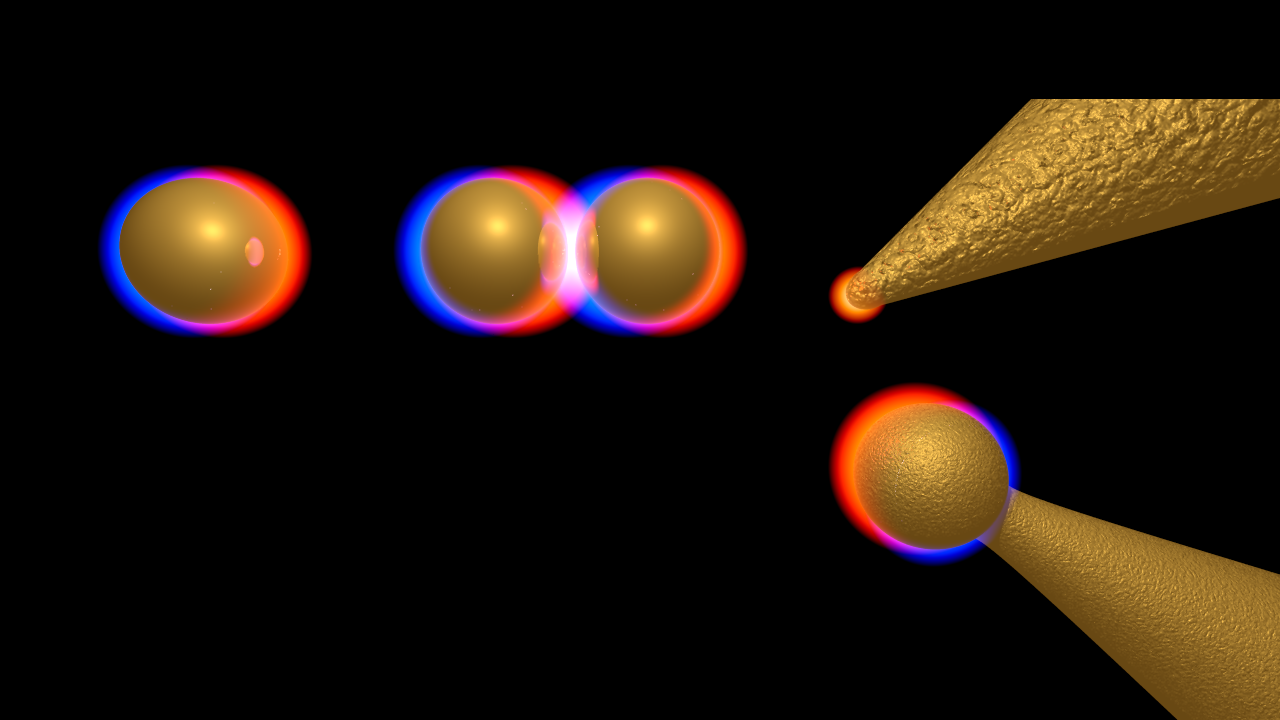
\includegraphics[width=\paperwidth, clip=true, trim=0 80 0 100]{figures/chapter_cover.png}}
%}}

% Why do this
As discussed in the theoretical background (section \ref{sec:tip_literature}) there has been little work to characterise and understand tips prior to applying them as near-field antennae. This has been one of the major {\color{red}driving forces/motivations} of this project. For this reason hyperspectral imaging is applied to laterally map the scattering from a tip with spectral confocally localised to infer a local optical response.
Understanding the properties of this response at the tip apex of single tips is not only important to determine how they will behave as near-field enhancers but also important in understanding their behaviour in the presence of another tip. By identifying the localised plasmonic behaviour of a set of tips, and comparing it with the underlying geometry, a better understanding can be gained when monitoring the hybridisation process.

% Summary of this chapter

\subimport{./}{hyperspectral_imaging}
\subimport{./}{tip_plasmonics_understanding}
\subimport{./}{nonplasmonic_tip_performance}
\subimport{./}{tip_plasmonics_applications}
\subimport{./}{tuneable_raman}

\section{Conclusions}

In conclusion, we have demonstrated a simple, fast method for the reliable growth of plasmonic spherical AuNP AFM tips. We showed this capability through measurements of dark-field scattering and SERS on controlled tip dimers at nanoscale separations.

\ifstandalone
\begin{singlespace}
\fontsize{8pt}{1em}\selectfont
\printbibliography[notcategory=fullcited]
\end{singlespace}
\fi

\end{document}